%!TEX root = ../../THESIS.tex

\section{Drawing and reading}

The previous section defined diagrams as a data structure based on lists of layers, in this section we define \emph{pictures of diagrams}.
Concretely, such a picture will be encoded in a computer memory as a bitmap, i.e. a matrix of colour values.
Abstractly, we will define these pictures in terms of topological subsets of the Cartesian plane.
We first recall the topological definition from Joyal's and Street's unpublished manuscript \emph{Planar diagrams and tensor algebra}~\cite{JoyalStreet88} and then discuss the isomorphism between the two definitions.
In one direction, the isomorphism sends a \py{Diagram} object to its drawing.
In the other direction, it reads the picture of a diagram and translates it into a \py{Diagram} object, i.e. its domain, codomain and list of layers.

A \emph{topological graph}, also called 1-dimensional cell complex, is a tuple $(G, G_0, G_1)$ of a Hausdorff space $G$ and a pair of a closed subset $G_0 \sub G$ and a set of open subsets $G_1 \sub P(G)$ called \emph{nodes} and \emph{edges} respectively, such that:
\begin{itemize}
\item $G_0$ is discrete and $G - G_0 = \bigcup G_1$,
\item each edge $e \in G_1$ is homeomorphic to an open interval and its boundary is contained in the nodes $\partial e \sub G_0$.
\end{itemize}
From a topological graph $G$, one can construct an undirected graph in the usual sense by forgetting the space $G$, taking $G_0$ as nodes and edges $(x, y) \in G_0 \times G_0$ for each $e \in G_1$ with $\partial e = \{ x, y \}$.
A topological graph is finite (planar) if its undirected graph is finite (planar, i.e. there exists some embedding embedding of the graph in the plane).

A \emph{plane graph} between two real numbers $a < b$ is a finite, planar topological graph $G$ with an embedding in $\R \times [a, b]$.
We define the domain $\dom(G) = G_0 \ \cap \ \R \times \{ a \}$, the codomain $\cod(G) = G_0 \ \cap \ \R \times \{ b \}$ as lists of nodes ordered by horizontal coordinates and the set $\boxes(G) = G_0 \ \cap \ \R \times (a, b)$.
We require that:
\begin{itemize}
    \item $G \ \cap \ \R \times \{ a \} = \dom(G)$ and $G \ \cap \ \R \times \{ b \} = \cod(G)$, i.e. the graph touches the horizontal boundaries only at domain and codomain nodes,
    \item every domain and codomain node $x \in G \ \cap \ \R \times \{ a, b \}$ is in the boundary of exactly one edge $e \in G_1$, i.e. edges can only meet at box nodes.
\end{itemize}
A plane graph is \emph{generic} when the projection on the vertical axis $p_1 : \R \times \R \to \R$ is injective on $G_0 \ - \ \R \times \{ a, b \}$, i.e. no two box nodes are at the same height.
From a generic plane graph, we can get a list $\boxes(G) \in G_0^\star$ ordered by height.
A plane graph is \emph{progressive} (also called \emph{recumbent} by Joyal and Street) when $p_1$ is injective on each edge $e \in G_1$, i.e. edges go from top to bottom and do not bend backwards.

From a progressive plane graph $G$, one can construct a directed graph by forgetting the space $G$, taking $G_0$ as nodes and edges $(x, y) \in G_0 \times G_0$ for each $e \in G_1$ with $\partial e = \{ x, y \}$ and $p_1(x) < p_1(y)$.
We can also define the domain and the codomain of each box node $\dom, \cod : \boxes(G) \to G_1^\star$ with
$\dom(x) = \{ e \in G_1 \ \vert \partial e = \{ x, y \}, p_1(x) < p_1(y) \}$ the edges coming in from the top and
$\cod(x) = \{ e \in G_1 \ \vert \partial e = \{ x, y \}, p_1(x) > p_1(y) \}$ the edges going out to the bottom, these sets are linearly ordered as follows.
Take some $\epsilon > 0$ such that the horizontal line at height $p_1(x) - \epsilon$ crosses each of the edges in the domain.
Then list $\dom(x) \in G_1^\star$ in order of horizontal coordinates of their intersection points, i.e. $e < e'$ if $p_0(y) < p_0(y')$ for the projection $p_0 : \R \times \R \to \R$ and $y^{(')} = e^{(')} \cap \{ p_1(x) - \epsilon \} \times \R$. Symmetrically we define the list of codomain nodes $\cod(x) \in G_1^\star$ with a horizontal line at $p_1 + \epsilon$.

A \emph{labeling} of progressive plane graph $G$ by a monoidal signature $\Sigma$ is a pair of functions from edges to objects $\lambda : G_1 \to \Sigma_0$ and from boxes to boxes $\lambda : \boxes(G) \to \Sigma_1$ which commutes with the domain and codomain.
From an lgpp (\emph{labeled generic progressive plane}) graph, one can construct a \py{Diagram}.

\begin{python}
{\normalfont Translation from labeled generic progressive plane graphs to \py{Diagram}.}
\vspace{5pt}
\hrule
\vspace{-15pt}
\begin{flalign*}
\py{def} \s & \py{read(} \s G, \s \lambda : G_1 \to \py{Ty}, \s \lambda : \boxes(G) \to \py{Box} \s \py{) -> Diagram:}&&\\
& \py{dom = [} \s \lambda(e) \s \py{for} \s x \in \dom(G) \s \py{for} \s e \in G_1 \s \py{if} \s x \in \partial e \s \py{]}&&\\
& \py{boxes = [} \s \lambda(x) \s \py{for} \s x \in \boxes(G) \s \py{]}&&\\
& \py{offsets = [len(} \s G_1 \ \cap \ \{ p_0(x) \} \times \R \s \py{) for} \s x \in \boxes(G) \s \py{]}&&\\
& \py{return decode(dom, zip(boxes, offsets))} &&
\vspace{-10pt}
\end{flalign*}
\hrule
\end{python}

In the other direction, there are many possible ways to draw a given \py{Diagram} as a lgpp graph, i.e. to embed its graph into the plane.
Vicary and Delpeuch \cite{DelpeuchVicary18} give a linear-time algorithm to compute such an embedding with the following disadvantage: the drawing of a tensor $f \otimes g$ does not necessarily look like the horizontal juxtaposition of the drawings for $f$ and $g$.
For example, if we tensor an identity with a scalar, the edge representing the identity will wiggle around the node representing the scalar.
DisCoPy uses a quadratic-time drawing algorithm with the following design decision: we make every edge a straight line and as vertical as possible.
We first initialise the lgpp graph of the identity with a constant spacing between each edge, then for each layer we update the embedding so that there is enough space for the output edges of the box before we add it to the graph.

\begin{python}
{\normalfont Outline of \py{Diagram.draw} from \py{Diagram} to \py{PlaneGraph}.}

\begin{minted}{python}
Embedding = dict[Node, tuple[float, float]]
PlaneGraph = tuple[Graph, Embedding]

def draw(self: Diagram) -> PlaneGraph:
    graph = diagram2graph(self)
    def make_space(scan: list[Node], box: Box, offset: int) -> float:
        """ Update the graph to make space and return the left of the box. """
    box_nodes = [Node('box', box, -1, j) for j, box in enumerate(self.boxes)]
    dom_nodes = scan = [Node('dom', x, i, -1) for i, x in enumerate(self.dom)]
    position = {node: (i, -1) for i, node in enumerate(dom_nodes)}
    for j, (left, box, _) in enumerate(self.layers):
        box_node, left_of_box = Node('box', box, -1, j), make_space(scan, box, offset)
        position[box_node] = (left_of_box + max(len(box.dom), len(box.cod)) / 2, j)
        for kind, epsilon in (('dom', -.1), ('cod', .1)):
            for i, x in enumerate(getattr(box, kind)):
                position[Node(kind, x, i, j)] = (left_of_box + i, j + epsilon)
        box_cod_nodes = [Node('cod', x, i, j) for i, x in enumerate(box.cod)]
        scan = scan[:len(left)] + box_cod_nodes + scan[len(left @ box.dom):]
    for i, x in enumerate(self.cod):
        position[Node('cod', x, i, len(self))] = (position[scan[i]][0], len(self))
    return graph, position
\end{minted}
\end{python}

Note that when we draw the plane graph for a diagram, we do not usually draw the box nodes as points.
Instead, we draw them as boxes, i.e. a box node $x \in \boxes(G)$ is depicted as the rectangle with corners $(l, p_1(x) \pm \epsilon)$ and $(r, p_1(x) \pm \epsilon)$ for $l, r \in \R$ the left- and right-most coordinate of its domain and codomain nodes.
In this way, we do not need to draw the in- and out-going edges of the box node: they are hidden by the rectangle.
The only exceptions are \emph{spider boxes} where we draw the box node (the head) and its outgoing edges (the legs of the spider) as well as \emph{cup and cap boxes} where we do not draw the box node at all, only its two outgoing edges which are drawn as Bézier curves to look like cups and caps respectively.
Spiders, cups and caps will be discussed, and drawn, in section~\ref{section:extra structure}.

\begin{example}
\begin{minted}{python}
circuit = sqrt2 @ Ket(0) @ Ket(0) >> H @ Id >> CX
circuit.draw(to_tikz=True)
\end{minted}
\end{example}

\begin{example}
The following spiral diagram is the cubic worst-case for interchanger normal form.
It is also the quadratic worst-case for drawing, at each layer of the first half we need to update the position of every preceding layer in order to make space for the output.

\begin{minted}{python}
x = Ty('x')
f, g = Box('f', Ty(), x @ x), Box('g', x @ x, Ty())
u, v = Box('u', Ty(), x), Box('v', x, Ty())
x[0]._name =  "\\py{x}"
for box in [f, g, u, v]: box._name = "\\py{" + box.name + "}"

def spiral(n: int) -> Diagram:
    diagram = u
    for i in range(n): diagram >>= Id(x ** i) @ f @ Id(x ** (i + 1))
    diagram >>= Id(x ** n) @ v @ Id(x ** n)
    for i in range(n): diagram >>= Id(x ** (n - i - 1)) @ g @ Id(x ** (n - i - 1))
    return diagram

spiral(3).draw(to_tikz=True, textpad=(0.2, 0.2), tikz_options="scale=1.666",
               path="WORK/TEX/THESIS/img/spiral.tikz")
\end{minted}
\ctikzfig{img/spiral}
\end{example}

Next, we define the inverse translation \py{graph2diagram}.

\begin{python}
{\normalfont Translation from \py{PlaneGraph} to \py{Diagram}.}

\begin{minted}{python}
def graph2diagram(graph: Graph, position: Embedding) -> Diagram:
    dom = Ty(*[node.label for node in graph.nodes if node.kind == 'dom' and node.j == -1])
    boxes = [node.label for node in graph.nodes if node.kind == 'box']
    scan, offsets = [Node('dom', x, i, -1) for i, x in enumerate(dom)], []
    for j, box in enumerate(boxes):
        left_of_box = position[Node('dom', box.dom[0], 0, j)][0]\
            if box.dom else position[Node('box', box, -1, j)][0]
        offset = len([node for node in scan if position[node][0] < left_of_box])
        box_cod_nodes = [Node('cod', x, i, j) for i, x in enumerate(box.cod)]
        scan = scan[:offset] + box_cod_nodes + scan[offset + len(box.dom):]
        offsets.append(offset)
    return decode(dom, zip(boxes, offsets))
\end{minted}
\end{python}

\begin{theorem}\label{theorem:graph2diagram(self.draw())}
\py{graph2diagram(self.draw()) == self} for all \py{self: Diagram}.
\end{theorem}

\begin{proof}
By induction on \py{n = len(self.layers)}.
If \py{not len(self.layers)} we get that \py{dom == self.dom} and \py{boxes == offsets == []}.
If the theorem holds for \py{self}, it holds for \py{self >> Layer(left, box, right)}.
Indeed, we have:
\begin{itemize}
\item \py{dom == self.dom and boxes == self.boxes + [box]}
\item \py{(x, Node('cod', self.cod[i], i, n)) in graph for i, x in enumerate(scan)}
\end{itemize}
Moreover, the horizontal coordinates of the nodes in \py{scan} are strictly increasing,
thus we get the desired \py{offsets == self.offsets + [len(left)]}.
\end{proof}

A deformation $f : G \to G'$ between two labeled plane graphs $G, G'$ is a continuous map $h : G \times [0, 1] \to \R \times \R$ such that:
\begin{itemize}
\item $h(G, t)$ is a plane graph for all $t \in [0, 1]$, $h(G, 0) = G$ and $h(G, 1) = G'$,
\item $x \in \boxes(G)$ implies $h(x, t) \in \boxes(h(G, t))$ for all $t \in [0, 1]$,
\item $h(G, t) \fcmp \lambda = \lambda$ for all $t \in [0, 1]$, i.e. the labels are preserved throughout.
\end{itemize}
A deformation is progressive (generic) when $h(G, t)$ is progressive (generic) for all $t \in [0, 1]$.
We write $G \sim G'$ when there exists some deformation $f : G \to G'$, this defines an equivalence relation.

\begin{theorem}\label{theorem:g2d then d2g}
For all lgpp graphs $G$, \py{Diagram.draw(graph2diagram(} $G$ \py{))} $\sim G$ up to generic progressive deformation.
\end{theorem}

\begin{proof}
By induction on the length of $\boxes(G)$.
If there are no boxes, $G$ is the graph of the identity and we can deform it so that each edge is vertical with constant spacing.
If there is one box, $G$ is the graph of a layer and we can cut it in three vertical slices with the box node and its outgoing edges in the middle.
We can apply the case of the identity to the left and right slices, for the middle slice we make the edges straight with a constant spacing between the domain and codomain.
Because $G$ is generic, we can cut a graph with $n > 2$ boxes in two horizontal slices between the last and the one-before-last box, then apply the case for layers and the induction hypothesis.
To glue the two slices back together while keeping the edges straight, we need to make space for the edges going out of the box.

This deformation is indeed progressive, i.e. we never bend edges we only make them straight.
It is also generic, i.e. we never move a box node past another.
\end{proof}

\begin{theorem}\label{theorem:d2g then g2d}
There is a progressive deformation $h : G \to G'$ between two lgpp graphs iff \py{graph2diagram(} $G$ \py{) == graph2diagram(} $G'$ \py{)} up to interchanger.
\end{theorem}

\begin{proof}
By induction on the number $n$ of \emph{coincidences}, the times at which the deformation $h$ fails to be generic, i.e. two or more boxes are at the same height.
WLOG (i.e. up to continuous deformation of deformations) this happens at a discrete number of time steps $t_1, \dots, t_n \in [0, 1]$.
Again WLOG at each time step there is at most two boxes at the same height, e.g. if there are two boxes moving below a third at the same time, we deform the deformation so that they move one after the other.
The list of boxes and offsets is preserved under generic deformation, thus if $n = 0$ then \py{graph2diagram(} $G$ \py{) == graph2diagram(} $G'$ \py{)} on the nose.
If $n = 1$, take \py{i: int} the index of the box for which the coincidence happens and \py{left: bool} whether it is a left or right interchanger, then \py{graph2diagram(} $G$ \py{).interchange(i, left) == graph2diagram(} $G'$ \py{)}.
Given a deformation with $n + 1$ coincidences, we can cut it in two time slices with $1$ and $n$ coincidences respectively then apply the cases for $n = 1$ and the induction hypothesis.

For the converse, a proof of \py{graph2diagram(} $G$ \py{) == graph2diagram(} $G'$ \py{)}, i.e. a sequence of $n$ interchangers, translates into a deformation with $n$ coincidences.
\end{proof}

We have established an isomorphism between the class of lgpp graphs (up to progressive deformation) and the class of \py{Diagram} objects (up to interchanger).
It remains to show that this actually forms an isomorphism of monoidal categories.
That is for every monoidal signature $\Sigma$, there is a monoidal category $G(\Sigma)$ with objects $\Sigma_0^\star$ and arrows the equivalence classes of lgpp graphs with labels in $\Sigma$.
The domain and codomain of an arrow is given by the labels of the domain and codomain of the graph.
The identity $\id(x_1 \dots x_n)$ is the graph with edges $(i, a) \to (i, b)$ for $i \leq n$ and $a, b \in \R$ the horizontal boundaries.
The tensor of two graphs $G$ and $G'$ is given by horizontal juxtaposition, i.e. take $w = \max(p_0(G)) + 1$ the right-most point of $G$ plus a margin and set $G \otimes G' = G \cup \{ (p_0(x) + w, p_1(x)) \ \vert \ x \in G' \}$.
The composition $G \fcmp G'$ is given by vertical juxtaposition and connecting the codomain nodes of $G$ to the domain nodes of $G'$.
That is, $G \fcmp G' = s^+(G) \cup s^-(G') \cup E$ for $s^\pm(x) = \big( p_0(x), \frac{p_1(x) \pm (b - a)}{2} \big)$ and edges $s^+(\cod(G)_i) \to s^-(\dom(G')_i) \in E$ for each $i \leq \len(\cod(G)) = \len(\dom(G'))$.

The deformations for the unitality axioms are straightforward: there is a deformation $G \fcmp \id(\cod(G)) \sim G \sim \id(\dom(G)) \fcmp G$ which contracts the edges of the identity graph, the unit of the tensor is the empty diagram so we have an equality $G \otimes \id(1) = G = \id(1) \otimes G$.
The deformations for the associativity axioms are better described by the following hand-drawn diagrams from Joyal and Street.

\begin{figure}[H]
\centering
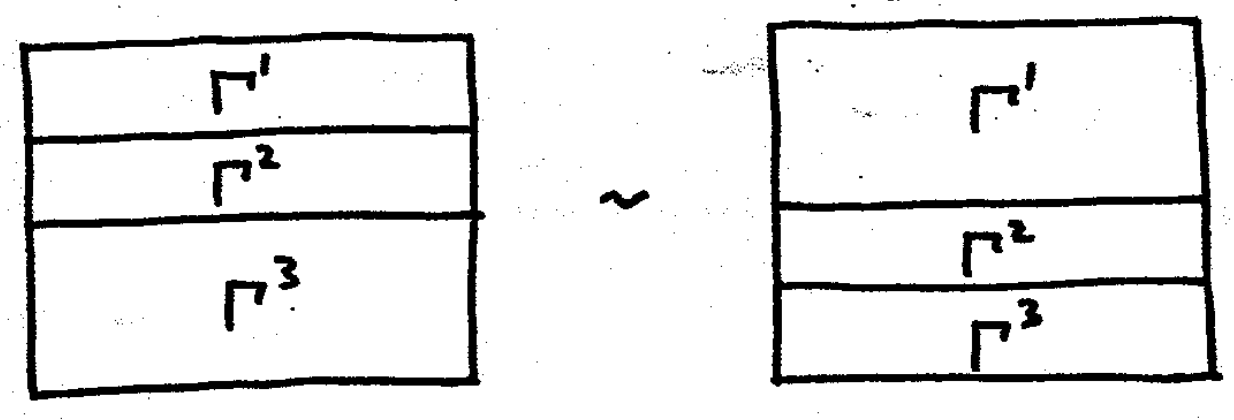
\includegraphics[scale=0.15]{img/tensor-assoc.png}
\qquad \quad 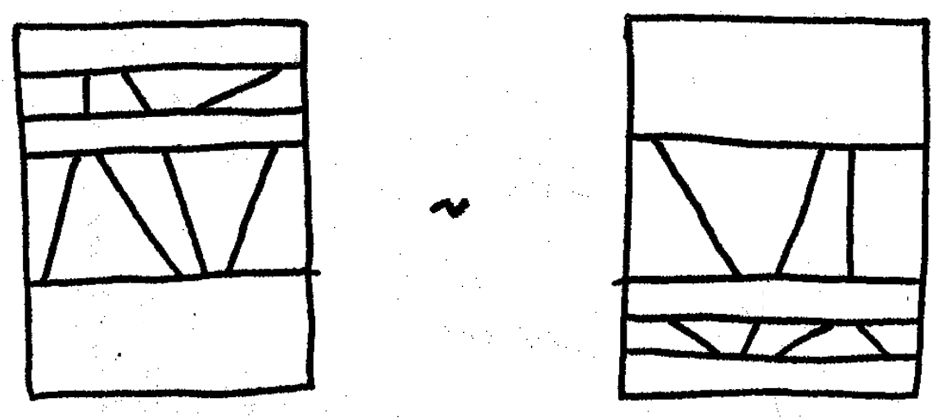
\includegraphics[scale=0.15]{img/compos-assoc.png}
\caption{Deformations for the associativity of tensor and composition.}
\end{figure}

The interchange law holds on the nose, i.e. $(G \otimes G') \fcmp (H \otimes H') = (G \fcmp H) \otimes (G' \fcmp H')$, as witnessed by the following hand-drawn diagram which is the result of both sides.

\begin{figure}[h]
\centering
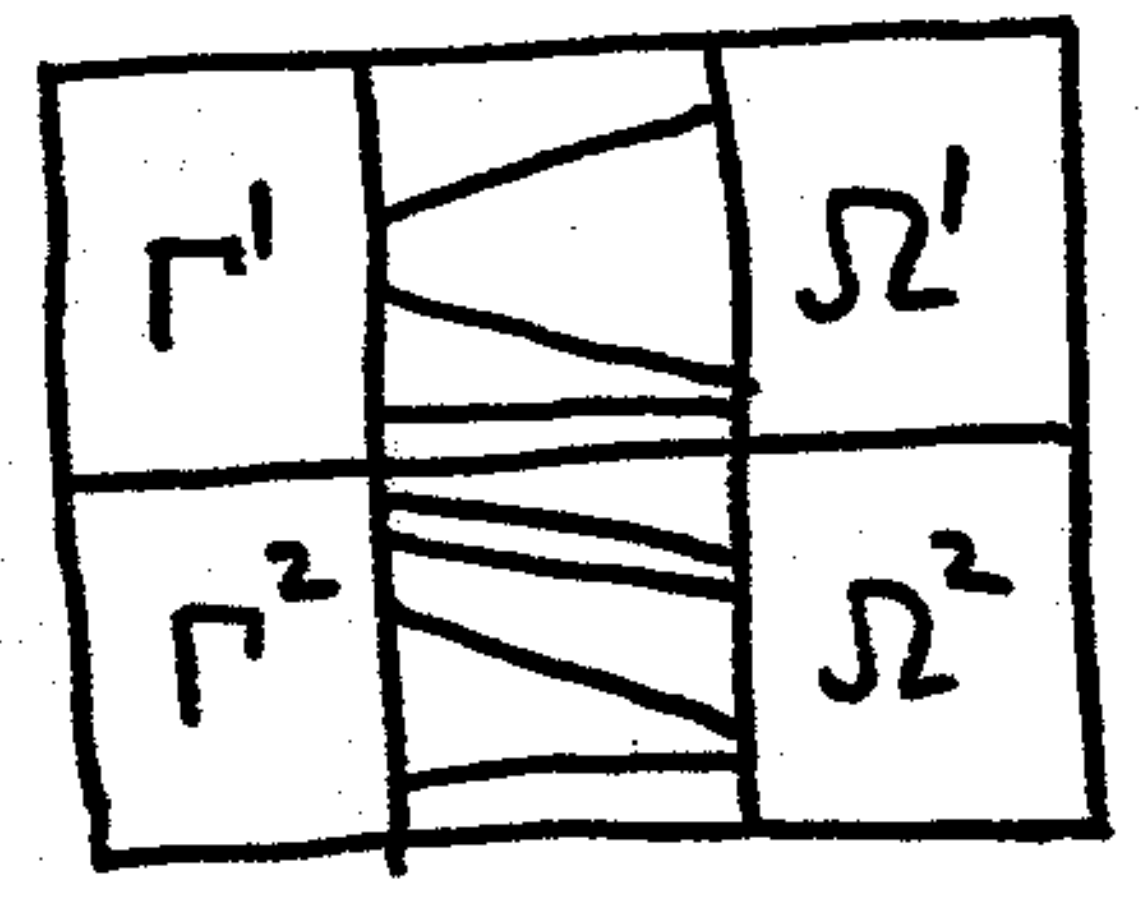
\includegraphics[scale=0.075]{img/interchange.png}
\caption{The graph of the interchange law.}
\end{figure}

Thus, we have defined a monoidal category $G(\Sigma)$.
Given a morphism of monoidal signatures $f : \Sigma \to \Gamma$, there is a functor $G(f) : G(\Sigma) \to G(\Gamma)$ which sends a graph to itself relabeled with $f \fcmp \lambda$, its image on arrows is given in listing~\ref{listing:G_of_f}.
Hence, we have defined a functor $G : \mathbf{Monsig} \to \mathbf{MonCat}$ which we claim is naturally isomorphic to the free functor $F : \mathbf{Monsig} \to \mathbf{MonCat}$ defined in the previous section.

\begin{python}\label{listing:G_of_f}
{\normalfont Implementation of the functor $G : \mathbf{Monsig} \to \mathbf{MonCat}$ on arrows.}

\begin{minted}{python}
SigMorph = tuple[dict[Ob, Ob], dict[Box, Box]]

def G(f: SigMorph) -> Callable[[Graph], Graph]:
    def G_of_f(graph: Graph) -> Graph:
        def relabel(node):
            if node.kind == 'box':
                return Node('box', f[1][node.label], node.i, node.j)
            return Node(node.kind, f[0][node.label], node.i, node.j)
        return Graph(map(relabel, graph.edges))
    return G_of_f
\end{minted}
\end{python}

\begin{theorem}
There is a natural isomorphism $F \simeq G$.
\end{theorem}

\begin{proof}
From theorems~\ref{theorem:g2d then d2g} and \ref{theorem:d2g then g2d}, we have an isomorphism between \py{Diagram} and \py{PlaneGraph} given by \py{d2g = Diagram.draw} and \py{g2d = graph2diagram}.
Now fix \py{F = lambda f: Functor(ob=f[0], ar=f[1])}.
Given a morphism of monoidal signatures \py{f: SigMorph} we have two naturality squares:
\begin{center}
    \begin{tikzcd}
    \py{Diagram} \ar{r}{\py{d2g}} \ar{d}[']{\py{F(f)}} &
    \py{PlaneGraph} \ar{d}{\py{G(f)}}\\
    \py{Diagram} \ar{r}{\py{d2g}} &
    \py{PlaneGraph}
    \end{tikzcd}
    \qquad \text{and} \qquad
    \begin{tikzcd}
    \py{PlaneGraph} \ar{r}{\py{g2d}} \ar{d}[']{\py{G(f)}} &
    \py{Diagram} \ar{d}{\py{F(f)}}\\
    \py{PlaneGraph} \ar{r}{\py{g2d}} &
    \py{Diagram}
    \end{tikzcd}
\end{center}
\end{proof}
